\documentclass[11pt, oneside]{article}
\usepackage[margin=1in]{geometry}
\geometry{letterpaper}
\usepackage{booktabs}
\usepackage{hyperref}
\usepackage{enumitem}
\usepackage{float}
\usepackage{caption}
\usepackage{subcaption}
\usepackage[numbers]{natbib}
\usepackage{graphicx}
\usepackage{amssymb}
\usepackage{amsmath}
\usepackage{array}
\usepackage{longtable}
\usepackage{xcolor}
\usepackage{tabularx}
\usepackage{setspace}
\usepackage{tikz}
\usetikzlibrary{positioning,fit,arrows.meta}
\hypersetup{
    colorlinks=true,
    linkcolor=blue,
    citecolor=blue,
    urlcolor=blue
}
% Red markers for facts the author still has to supply. None may remain in the submitted PDF.
\newcommand{\todo}[1]{\textcolor{red}{[TODO: #1]}}
\captionsetup{font=small,skip=3pt}
\setlength{\textfloatsep}{8pt plus 2pt minus 2pt}
\setlength{\floatsep}{6pt plus 2pt minus 2pt}
\setlength{\intextsep}{6pt plus 2pt minus 2pt}
% ============================================================
% TITLE BLOCK --- students must keep this format
% Filename of the compiled PDF must be:
% CS781-CP-[Firstname]-[Lastname]-[RollNo]-report.pdf
% ============================================================
\title{CS781 Capstone Project:\\
In-House Legal Intelligence System}
\author{
    Aryan Kumar  \\
    261110012 \\
    {\tt aryank26@iitk.ac.in}\\
    Indian Institute of Technology Kanpur (IIT Kanpur)\\
    Code: \url{https://github.com/akode2803/CS781-Legal-LLM-Capstone}
}
\date{}
\begin{document}
\maketitle
\begin{abstract}
Law firms cannot send their confidential judgments to hosted APIs, therefore we built a self-hosted Indian legal NLP stack under a 300M-parameter cap. I first trained four 63--67M-parameter decoders on about 125M legal tokens using only the course data, and then retrained three 214M-parameter models on 4.0B tokens each: a GQA decoder, a Hymba-style hybrid mixing attention with Mamba-2 heads, and an MLM encoder. For each phase task (entity recognition, rhetorical roles, judgment prediction, statute identification, summarization and prior case retrieval), I fine-tuned one of those checkpoints using full fine-tuning, LoRA, LoRMA, IA$^3$, partial tuning or distillation. There are three key takeaways: scaling up pretraining helps to a degree, as the 214M models outperformed the 67M ones by about 0.05 macro-F1 on statutes; the model backbones as well as tuning methods were essentially tied within seed and test noise, with LoRMA performing as well as full fine-tuning at about half the memory; and in the final phase, lexical baselines were very difficult to beat, with word n-gram overlap driving most of our retrieval score.
\end{abstract}
% ============================================================
\section{Competition Result}
% ============================================================
\noindent
\textbf{Codabench username:} a\_261110012
\hfill
\textbf{Roll number:} 261110012
\medskip

\noindent
The table below lists our best valid score in each phase.
\begin{table}[H]
\centering\small
\begin{tabular}{clccc}
\toprule
Phase & Task & Primary metric (value) & Rank & Valid submissions \\
\midrule
1 & Legal LM Pretraining & BERTScore-F1 0.8298 & 84 of 142 & 11 (7 distinct) \\
2 & Legal NER & strict macro-F1 0.5443 & 52 of 132 & 7 (6 distinct) \\
3 & Rhetorical role prediction & macro-F1 0.4642 & 89 of 131 & 8 \\
4 & Court judgment prediction & macro-F1 0.5992 & 122 of 130 & 18 \\
5 & Legal statute identification & macro-F1 0.3965$^\ast$ & 41 of 129 & 14 \\
6 & Abstractive summarization & BERTScore-F1 0.8450 & 42 of 124 & 12 \\
7 & Prior Case Retrieval (PCR) & Micro-F1@7 0.4938 & 8 of 121 & 17 \\
\bottomrule
\end{tabular}
\\[2pt]{\footnotesize $^\ast$A later Phase 5 submission scored 0.4180 but is marked ``Failed'' and is not on the leaderboard.}
\end{table}
\noindent
\textbf{Total valid Codabench submissions across all phases:} 87
\quad
\textbf{Date ranks were recorded:} 8 November 2026
\medskip

\noindent We met the minimum of four distinct submissions in every phase.
% ============================================================
\section{Introduction and Problem Description}
% ============================================================
As client records are confidential, a law firm has to run language models on its own hardware, trained only on data it owns. We built that stack here for Indian law in seven phases: pretrain a 50M--300M-parameter model from scratch and continue on 128-word judgment prompts (Phase 1, BERTScore F1 \cite{zhang2020bertscore}), extract 12 types of entity span with exact character offsets (Phase 2, strict macro-F1), label sentences with 13 rhetorical roles (in Phase 3, macro-F1) \cite{kalamkar2022corpus}, predict whether an appeal is allowed (in Phase 4, macro-F1) \cite{malik2021ildc}, identify which of 100 statutes a case invokes (Phase 5, macro-F1), write a judgment summary (in Phase 6, BERTScore F1) and retrieve the prior cases a judgment cites (in Phase 7, Micro-F1 over seven predictions).

In line with the rules, no pretrained model or external corpus may be used, so all the neural models are derived from our own Phase 1 checkpoints. Colab compute was used throughout (model size and token budget held constant) and the judgments (median 4,200 tokens in Phase 4) ran far longer than the 512 or 2,048 tokens our models actually consumed. We tracked four questions throughout: does more pretraining help? do attention variants or a state-space hybrid help? which tuning method transfers best? and how far does a neural model beat a lexical baseline? We built and submitted every phase end to end, used the course tokenizer rather than training our own, and did not use the Phase 7 citation traces (Section~\ref{sec:preproc}).
% ============================================================
\section{Data Analysis and Preprocessing}
% ============================================================
\subsection{Sources and official splits}
We used only the official configurations of \texttt{Exploration-Lab/CS-781-Capstone} (Table~\ref{tab:data}).

\begin{table}[H]
\centering\footnotesize
\setlength{\tabcolsep}{3pt}
\caption{Splits and design-relevant statistics (our counts). Lengths are in course-BPE tokens unless marked as words.}
\label{tab:data}
\begin{tabularx}{\textwidth}{c>{\raggedright\arraybackslash}p{3.1cm}>{\raggedright\arraybackslash}X>{\raggedright\arraybackslash}p{4.2cm}}
\toprule
Phase & Train / dev / test & Statistics & Design consequence \\
\midrule
1 & 19.2 GB text & High Courts 10.67 GB, tribunals 6.48, Supreme Court 1.32, Acts 0.73; 3.7--4.0 characters per token; 4.3--4.6B tokens after cleaning & One pass in natural proportions; 4.0B-token budget, about 19 tokens per parameter \\
2 & 70 docs (2 folds) / -- / 35 docs & Median 4,488 words; 120 entities per document. DATE 18.8\%, STAT 15.0\%, PREC 14.1\%, \dots, counsel and witnesses about 2\% each. Median span 2 words (p95 9); no overlapping spans; 26 strings carry two labels (``Union of India'') & BIO tags over words; CRF with legal transitions; windows over the full text \\
3 & 80 / 10 / 10 docs (16,845 / 2,142 sentences) & 13 roles, CL and IT domains. ArgumentPetitioner is 24.6\% of dev CL sentences against 9.2\% in train; 17.6\% (CL) and 22.2\% (IT) of sentences exceed 63 tokens & Neighbouring-sentence context; square-root class weights \\
4 & 31,677 / 994 / 1,517 & Train is 41\% accepted, dev 50\%. Mean 5,500 tokens (median 4,200, p90 10,000). TF-IDF on the last third scores 0.629, the first third 0.576 & Read the last eight 512-token chunks \\
5 & 42,513 / 10,155 / 13,019 & 100 statutes with 272--11,731 training cases each; 3.7 per case (max 31). Mean 1,909 tokens, median 768 & Eight chunks cover 87\% of cases; per-statute thresholds \\
6 & 7,030 / 200 held out / 100 & Judgments: median 3,129 words (p90 7,855). Summaries: median 638 words, ratio 0.217; 11\% of summary sentences occur verbatim & Abstractive decoder; length set as a ratio of the input \\
7 & 827 / 118 / 237 queries; pools 4,320 / 1,023 / 1,727 & Gold per dev query: mean 8.2, median 5, max 92; a perfect ranking scores 0.618. Gold is older than the query in 352 of 352 dated pairs & Lexical first stage; date filter; self-matches removed \\
\bottomrule
\end{tabularx}
\end{table}

\subsection{Corpus statistics that actually informed design}
In \textbf{Phase 1}, High Court and tribunal cases make up 89\% of the corpus; initial runs sampled equally and only got 2.7\% of the data, therefore our restart did one pass in natural proportions to spend the budget on tokens rather than balance. In \textbf{Phase 3}, dev has only 10 docs and its CL portion is missing Dissent and PrecedentNotReliedUpon, so dev macro-F1 averages the present classes and swings in points with one document. For \textbf{Phase 4}, every dev case appears twice (1,988 rows) and 5,710 duplicates were removed from train; as the latter third of a case is most predictive we keep the last chunks. In \textbf{Phase 5}, a 43-fold gap in statute frequency makes one global threshold too high for rare statutes, and in \textbf{Phase 7} queries citing one or two gold cases cap precision near 0.2 whereas those citing more than seven cap recall.

\subsection{Preprocessing}\label{sec:preproc}
Every stage uses the frozen course BPE tokenizer (vocabulary 32,768) without lowercasing or normalization, and prior to Phase 1 pretraining we dropped empty records, documents under 200 chars and exact duplicates; to prevent leakage, we also took token 16-gram fingerprints of the Phase 4 and 5 dev and test sets and removed the 5,470 corpus documents sharing 20 or more of those (we never did that check on Phases 2 and 3). For \textbf{Phase 2 offsets} the tokenizer gives us the Unicode character span (end exclusive) of each BPE piece. As we never normalize the text at all, the predicted words map directly back to character offsets and the annotation checks confirmed 0 mismatches in 8,393 gold entities. \textbf{Phase 3} just takes the input sentence lists as they are and caps all sentences at 63 tokens. In \textbf{Phases 4 and 5} we split each case into 512-token chunks and keep at most eight (the last eight in Phase 4, eight evenly spaced in Phase 5). For \textbf{Phase 6} we fill our document budget (1,536 tokens in the final system) with the first three quarters from the start of the judgment and the last quarter from the end, with the remainder going to the summary. In \textbf{Phase 7} each query and candidate gets one 512-token excerpt made of the 96-token opening plus sentences sharing the most rare word 4-grams with the other document. The organizers mask citations as \texttt{<CITATION>} but traces remain. Matching those directly took dev F1 from 0.4603 to 0.4747, but as that exploits the gaps in the masking and improves no model we never submitted that.
% ============================================================
\section{Approach and Model Evolution}
% ============================================================
\subsection{Phase-1 foundation model}
For our \textbf{first models}, I started with four 12-layer causal decoders (width 512, 8 heads, SwiGLU FFN of 2,048 \cite{shazeer2020glu}, RMSNorm \cite{zhang2019rmsnorm}, RoPE \cite{su2024roformer}, context 2,048) that differed only in attention and normalization, namely multi-head pre-norm (67.4M), GQA with 2 key--value heads \cite{ainslie2023gqa} (62.7M), latent attention \cite{deepseek2024v2} (67.0M) and multi-head post-norm (67.4M); after a WikiText stage we trained them on about 125M legal tokens with sources sampled equally for Phases 2 to 5, including our Task 1 runs (Table~\ref{tab:variants}) where greedy decoding with repeated token 4-grams blocked did best (0.8298 BERTScore), though the post-norm model repeated itself in Task 1 and collapsed under partial fine-tuning later, and no model beat TF-IDF in Phases 4 and 5, so when a Phase 4 frozen-feature probe gave 0.562 dev macro-F1 for the old GQA model against 0.514 for random weights and 0.612 for TF-IDF we took that as under-training and restarted on 27 October.

For the \textbf{final models}, we trained three models of the same size on the same 4.0B tokens in identical order so their losses compare directly (Table~\ref{tab:arch}, Figure~\ref{fig:arch}): the GQA decoder has 16 layers, width 1,024, 16 query and 4 key--value heads with a SwiGLU FFN of 2,816, and the hybrid is based on Hymba \cite{dong2024hymba} so in each layer eight GQA heads and eight Mamba-2 SSD heads \cite{dao2024mamba2} take the normalized input in parallel, each branch output is normalized and scaled per channel by a learned vector, and both are concatenated before the output projection. As we left out Hymba's meta tokens, sliding-window attention and cross-layer key--value sharing, we call it Hymba-style and checked our plain-PyTorch SSD scan against the step-by-step recurrence; the encoder reuses the decoder code with bidirectional attention and a 30\% masked-language-model loss \cite{devlin2019bert} on 512-token windows, and after checking the parameter cap by summing sizes at construction (213.9M, 215M and 213.9M) we dropped the latent-attention decoder when benchmarking showed 56k tokens/s against 130k for GQA.

All three runs use AdamW \cite{loshchilov2019adamw} ($\beta=(0.9,0.95)$, weight decay 0.1 on matrices only), a peak learning rate of $6\times10^{-4}$ with 300 warm-up steps and cosine decay to $6\times10^{-5}$, clipping gradients at 1.0, bf16 and batches of 524,288 tokens for 7,629 steps; as data order is a fixed function of the step, any killed run resumes on the exact unseen data, and our budget of about 19 tokens per parameter follows the compute-optimal ratio \cite{hoffmann2022chinchilla}.

\begin{table}[H]
\centering\small
\setlength{\tabcolsep}{4pt}
\caption{Final Phase 1 models, all trained on the same 4.0B tokens. The encoder's masked-LM loss is not comparable with the causal losses.}
\label{tab:arch}
\resizebox{\textwidth}{!}{\begin{tabular}{lccccc}
\toprule
Model & Shape & Params & Speed (tokens/s) & Wall clock & Final val.\ loss \\
\midrule
GQA decoder & 16 layers, $d$ 1024, 16/4 heads, FFN 2816 & 213.9M & 130k & 8.6 h & 1.236 \\
Hybrid & 16 layers, 8 GQA + 8 SSD heads, FFN 2688 & 215M & 113k & 10.0 h & 1.189 \\
MLM encoder & as GQA, bidirectional, window 512 & 213.9M & 172k & 6.5 h & 0.686 (MLM) \\
\bottomrule
\end{tabular}}
\end{table}

\begin{figure}[H]
\centering
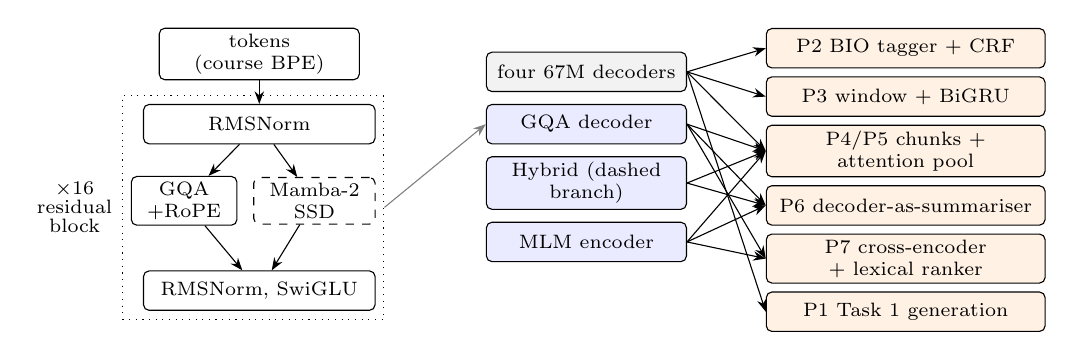
\begin{tikzpicture}[font=\scriptsize, node distance=3mm and 4mm,
  box/.style={draw, rounded corners=2pt, align=center, inner sep=2pt, minimum height=5mm},
  ck/.style={box, fill=blue!8}, hd/.style={box, fill=orange!10, text width=34mm},
  ar/.style={-{Stealth[length=1.6mm]}}]
\node[box, text width=24mm] (in) {tokens (course BPE)};
\node[box, text width=28mm, below=of in] (n1) {RMSNorm};
\node[box, text width=12mm, below left=4mm and -12mm of n1] (att) {GQA\\+RoPE};
\node[box, text width=14mm, right=2mm of att, dashed] (ssd) {Mamba-2\\SSD};
\node[box, text width=28mm, below=16mm of n1] (ffn) {RMSNorm, SwiGLU};
\node[draw, dotted, inner sep=3pt, fit=(n1)(att)(ssd)(ffn), label={[align=center]left:$\times16$\\[-1pt]residual\\[-1pt]block}] (blk) {};
\draw[ar] (in) -- (n1); \draw[ar] (n1) -- (att); \draw[ar] (n1) -- (ssd);
\draw[ar] (att) -- (ffn); \draw[ar] (ssd) -- (ffn);
\node[ck, right=14mm of n1, text width=24mm] (gqa) {GQA decoder};
\node[ck, below=1.5mm of gqa, text width=24mm] (hyb) {Hybrid (dashed branch)};
\node[ck, below=1.5mm of hyb, text width=24mm] (enc) {MLM encoder};
\node[ck, above=1.5mm of gqa, text width=24mm, fill=gray!10] (old) {four 67M decoders};
\node[hd, right=10mm of old, yshift=3mm] (p2) {P2 BIO tagger + CRF};
\node[hd, below=1mm of p2] (p3) {P3 window + BiGRU};
\node[hd, below=1mm of p3] (p4) {P4/P5 chunks + attention pool};
\node[hd, below=1mm of p4] (p6) {P6 decoder-as-summariser};
\node[hd, below=1mm of p6] (p7) {P7 cross-encoder + lexical ranker};
\node[hd, below=1mm of p7] (p1) {P1 Task 1 generation};
\draw[ar] (old.east) -- (p2.west); \draw[ar] (old.east) -- (p3.west); \draw[ar] (old.east) -- (p4.west);
\draw[ar] (gqa.east) -- (p4.west); \draw[ar] (gqa.east) -- (p6.west); \draw[ar] (gqa.east) -- (p7.west); \draw[ar] (old.east) -- (p1.west);
\draw[ar] (hyb.east) -- (p4.west); \draw[ar] (hyb.east) -- (p6.west);
\draw[ar] (enc.east) -- (p4.west); \draw[ar] (enc.east) -- (p6.west); \draw[ar] (enc.east) -- (p7.west);
\draw[ar, gray] (blk.east) -- (gqa.west);
\end{tikzpicture}
\caption{Left: the shared block; the hybrid adds the dashed SSD branch beside attention. Right: which checkpoint each phase fine-tunes. Phase 4 and 5 arrows from the new models refer to the probe (Phase 4) and the final runs (Phase 5).}
\label{fig:arch}
\end{figure}

\subsection{Transfer protocol (Phases 2--7)}
In the downstream phases every neural model puts a small task head on a Phase 1 checkpoint (only the TF-IDF baselines and the Phase 7 ranker are not language models), and to see how much of the backbone needed updating (Section~\ref{sec:ablations}) I compared updating all weights in full fine-tuning against updating only the top blocks in partial tuning, learning only per-channel scaling vectors with IA$^3$ \cite{liu2022ia3}, adding a trainable low-rank update $W+BA$ to the query and value projections with LoRA \cite{hu2022lora} (rank 8 in Phase 3, 16 later), or applying that low-rank factor multiplicatively as $(I+BA)W$ with LoRMA \cite{bihany2025lorma} so existing directions are rescaled rather than added to, alongside distilling \cite{hinton2015distilling} a student that keeps every other block of the checkpoint (6 of 12 or 8 of 16) on a mix of gold labels and the teacher's softened outputs (temperature 2, weight 0.5).

\subsection{Phase 2 - Legal NER}
Here we cast NER as BIO tagging over words (25 tags), cutting each judgment into 512-token windows (stride 384), representing each word by the backbone state of its last BPE piece, and running a BiLSTM over those states for tag scores before Viterbi decoding in a CRF \cite{lafferty2001crf} whose transitions block invalid moves (an I tag after O or after another type), so every predicted span comes out well formed from first to last character. Across our runs I fine-tuned the GQA and MHA pre-norm checkpoints, ran GQA for 15 epochs, tried LoRMA and a 6-layer distilled student, and equally averaged the two models' tag scores and CRF weights, though I also coded a span classifier over candidates up to 32 tokens that we never submitted.

\subsection{Phase 3 - Rhetorical role prediction}
Here I packed a window of 12 consecutive sentences (each capped at 63 tokens) with three context sentences on each side into one sequence of at most 512 tokens, taking the mean and last token states of every sentence and passing them through an MLP, a bidirectional GRU over the window and a linear role head with square-root inverse-frequency class weights so a single model covers both domains, and beside a sentence-only ablation that encodes every sentence alone I tested full fine-tuning (MHA), LoRMA (GQA), LoRA (MLA), IA$^3$ (MHA), position features and a distilled LoRMA student taught by the MHA model, whereas document-level transition priors and CRF layers on cheap features did not help (Section~\ref{sec:errors}).

\subsection{Phase 4 - Court judgment prediction}
Here I encoded the last eight 512-token chunks of each case separately and pooled them with learned attention scores into one case vector for a binary head, submitting every run at threshold 0.5 as well as a dev-tuned threshold across nine runs that cross backbone with tuning method, a 6-layer distilled student, and an equal-weight ensemble of runs 1 to 4 picked before test.

\subsection{Phase 5 - Legal statute identification}
Here our Phase 4 encoder takes eight evenly spaced chunks to feed 100 sigmoid heads with binary cross-entropy and square-root positive weights; as separate thresholds $t_k$ overfit on rare statutes, we pull them towards the global threshold $g$:
\begin{equation}
\theta_k = \lambda_k t_k + (1-\lambda_k)\, g, \qquad \lambda_k = \frac{n_k}{n_k+m},
\end{equation}
where $n_k$ counts training cases with statute $k$ so $m=0$ gives per-statute thresholds and $m\to\infty$ gives one global threshold, and after picking $m$ via five two-fold cross-fits on dev (always predicting at least one statute) we averaged six neural runs (three new models, two seeds) with a TF-IDF linear SVM weighted at 0.9.

\subsection{Phase 6 - Abstractive summarization}
Here I trained each model as a decoder-only summarizer over ``document, end token, `Summary:', summary'' with loss only on summary tokens (running the encoder as a prefix language model, bidirectional over the document and causal over the summary), set target length to 0.18 of the document's word count clipped to 200--700 words decoded by 4-beam search with no repeated 3-gram, and gave the document 1,536 of the 2,048 context tokens so about 510 remain for the summary, which is about the window BERTScore scores (Section~\ref{sec:errors}), with no post-training nor alignment.

\subsection{Phase 7 - Prior Case Retrieval (PCR)}\label{sec:pcr}
Our retrieval pipeline works in three stages \cite{nogueira2019passage}: first, a hashed word 4-gram overlap score (document-frequency cap 0.05, length normalization 0.6) ranks the pool after dropping self-matches and cases dated after the query, getting 0.4603 dev F1 against 0.101 for unigram BM25 \cite{robertson2009bm25} because citing judgments quote the cases they cite. Second, a gradient-boosted ranker \cite{pedregosa2011sklearn,ke2017lightgbm} rescores the top 50 using 27 features, including overlap taken only from query sentences near a \texttt{<CITATION>} tag, using where a citation sits, not which case it was. Finally, Phase 1 rerankers read the paired excerpts (Section~\ref{sec:preproc}) of each top-50 candidate together and score the pair with a linear head on the token mean (encoder) or last token (GQA), trained with softmax cross-entropy over one gold case and seven negatives from the lexical top 40; the combined score is
\begin{equation}
s(q,c) = z_q\big(\mathrm{logit}\,r(q,c)\big) + 0.2\cdot\tfrac{1}{3}\textstyle\sum_{m=1}^{3} z_q\big(n_m(q,c)\big),
\end{equation}
where $z_q$ standardizes within a query, $r$ is the ranker and $n_m$ are three rerankers (a fully fine-tuned encoder on plain excerpts, plus a fully fine-tuned encoder and a GQA LoRMA model on query excerpts filled first from citing sentences); four things I tried failed, namely feeding the neural score as a ranker feature, retraining on train plus dev, four-epoch training (0.95 train top-1 accuracy as dev neural F1 dropped near 0.32), and averaging eight rerankers (0.4932 on test).
% ============================================================
\section{Experiments and Implementation Details}
% ============================================================
\subsection{Compute and training protocol}
All runs were trained on Colab; for downstream tasks I used AdamW with warm-up and decay, bf16, separate learning rates on the backbone, adapters and head, and a wall-clock cap with resumable checkpoints, keeping the epoch with best dev macro-F1 in Phases 3 to 5, lowest validation loss in Phase 6, and highest standalone reranker dev F1 in Phase 7 (Table~\ref{tab:hparams}).

\begin{table}[H]
\centering\footnotesize
\setlength{\tabcolsep}{3pt}
\caption{Hyperparameters of the final model in each phase. LR: backbone / adapter / head.}
\label{tab:hparams}
\resizebox{\textwidth}{!}{\begin{tabular}{lccccccc}
\toprule
 & P1 & P2 & P3 & P4 & P5 & P6 & P7 \\
\midrule
Model & GQA & GQA + MHA & GQA LoRMA & 4-run ens. & 3 models & hybrid & 2 enc.\ + GQA \\
Parameters (M) & 213.9 & 62.7 + 67.4 & 62.7 & 39.9--67.4 & 214--215 & 215 & 213.9--214.6 \\
Context length & 2048 & 512, stride 384 & $\le$512 & 8$\times$512 & 8$\times$512 & 2048 & 512+512 \\
Peak LR & 6e-4 & 1e-5/--/1e-3 & --/1e-3/1e-3 & 3e-5/1e-3/5e-4 & 5e-5/--/1e-3 & 3e-5 & 2e-5 (3e-4)/1e-4 \\
Batch $\times$ accum. & 32$\times$8 seq. & 1 window & 8 windows & 4$\times$2 cases & 4$\times$4 cases & 2$\times$8 & 8 pairs$\times$4 \\
Epochs / steps & 7,629 steps & best of $\le$20: 6, 1 & 8 & 5$\times$2,000 cases & 4$\times$12,000 cases & 2 & 2 or 4 \\
Dropout & 0 & 0.2 & 0.1 & 0.1 & 0.1 & 0 & 0 \\
Decoding / threshold & greedy, no-rep.\ 3 & BIO, Viterbi & argmax & dev-tuned & shrunk, $m{=}30$ & 4 beams, no-rep.\ 3 & top 7 \\
\bottomrule
\end{tabular}}
\end{table}

\subsection{Local evaluation}
Phases 3, 4, 5 and 7 have labeled dev splits (with Phase 4 deduplicated to 994 cases) and in Phase 6 we held out 200 training docs and scored 100 with the organizers' BERTScore setup, scoring Phase 5 per-statute thresholds via two-fold cross-fit and comparing Phase 7 runs using a paired bootstrap over queries; local and Codabench numbers diverged twice, as Phase 4 dev-tuned thresholds overstated test by 2.5 points on average (beating threshold 0.5 by only 0.12 points on test) and Phase 6 test ran 0.005--0.008 below validation in every submission, probably because test references are longer (932 against 751 words) even though gains carried over, whereas Phase 7 test stayed within about 0.006 of dev and Phase 3 dev (10 docs) did not rank runs reliably (Section~\ref{sec:errors}).

\subsection{Ablations and controlled comparisons}\label{sec:ablations}
For the \textbf{adaptation method}, Table~\ref{tab:methods} puts together all runs varying how the checkpoint is tuned, showing that within each phase the differences sit inside noise (test standard error is about $\pm0.013$ in Phase 4, with seed spread 0.003--0.007 in Phase 5 and 0.0097 in Phase 7) and the Phase 4 controls holding architecture fixed (runs 2, 7, 8) or method fixed (runs 2, 9, 10) show no difference on test; LoRMA matched full fine-tuning in Phases 4, 6 and 7 by keeping under 1\% of weights trainable at about half the memory (6.2 against 12.0 GB in Phase 7), whereas partial tuning of the post-norm model collapsed in every phase and our distilled student matched its teacher in Phase 4 (0.5766 against 0.5776 dev) with 41\% fewer parameters and 2.2 times faster inference even though it lost a third of standalone quality in Phase 7.

\begin{table}[H]
\centering\footnotesize
\setlength{\tabcolsep}{4pt}
\caption{Adaptation methods across phases. Backbones: G = GQA, M = MHA pre-norm, P = MHA post-norm, L = latent attention (old 67M models in P3--P5), E = encoder (new 214M models in P6--P7, with G). P3: dev macro-F1. P4: test macro-F1 at threshold 0.5. P5: old models, dev macro-F1, global threshold. P6: test BERTScore. P7: dev neural F1 when the model alone ranks the top 50 (chance 0.112).}
\label{tab:methods}
\begin{tabular}{lccccc}
\toprule
Method & P3 & P4 & P5 & P6 & P7 \\
\midrule
Full fine-tuning & 0.4622 M & 0.5805 M, 0.5838 G & 0.305 M & 0.8350 G, 0.8345 E & 0.3168 G, 0.3391 E \\
LoRA & 0.4457 L & 0.5665 L, 0.5648 G & 0.279 L & 0.8303 G & 0.3135 G \\
LoRMA & 0.4478 G & 0.5854 G, 0.5854 M & 0.268 G & 0.8330 G & 0.3335 G \\
IA$^3$ & 0.4153 M & -- & -- & -- & 0.3002 G \\
Partial (top blocks) & -- & 0.4877$^\dagger$ P & 0.088 P & -- & 0.3168 G \\
Distilled student & 0.4942$^\ddagger$ G & 0.5846 G (6 of 12) & 0.261 G & 0.8299 G (8 of 16) & 0.2079 G (8 of 16) \\
\bottomrule
\end{tabular}
\\[2pt]{\footnotesize $^\dagger$Dev-tuned threshold. $^\ddagger$LoRMA student with all 12 blocks, taught by the MHA model: distillation as regularisation, not compression.}
\end{table}

On \textbf{pretraining scale and architecture}, scaling from the 67M models to the 214M ones pushed Phase 5 dev macro-F1 from 0.305 to 0.354--0.363, the biggest jump in the project, and on the frozen probe it went from 0.562 (old GQA) to 0.589 (new GQA) and 0.602 (hybrid at 75\% of pretraining), still below TF-IDF (0.612); downstream, the three new models were basically tied, as Phase 5 dev cross-fit came out to 0.3703, 0.3667 and 0.3637 for encoder, hybrid and GQA (within a seed spread of up to 0.007) and on Phase 6 test the hybrid got 0.8356 against 0.8350 for GQA.

In our \textbf{Phase 7 controls}, Table~\ref{tab:p7controls} varies one factor of the encoder reranker at a time, where we count a difference as real only if its interval excludes zero and exceeds the seed spread.

\begin{table}[H]
\centering\footnotesize
\caption{Phase 7 one-factor controls on dev, one seed each. Neural F1 as in Table~\ref{tab:methods}; intervals from a paired query bootstrap. Hits: gold cases in the top 7 when the run is added to the ranker at weight 0.2 (ranker alone 445). $^\ast$Mean pooling, hard negatives, listwise loss.}
\label{tab:p7controls}
\begin{tabular}{lcccc}
\toprule
Run & Neural F1 & Difference [95\% interval] & AUC (top 50) & Hits \\
\midrule
Encoder baseline$^\ast$ & 0.3391 & -- & 0.771 & 447 \\
Pairwise loss & 0.3324 & $-0.0067$ [$-0.0173$, 0.0035] & 0.765 & 447 \\
Random negatives & 0.4002 & $+0.0611$ [0.0363, 0.0886] & 0.881 & 442 \\
Last-token pooling & 0.3079 & $-0.0311$ [$-0.0501$, $-0.0135$] & 0.747 & 444 \\
Frozen backbone, head only & 0.2379 & $-0.1012$ [$-0.1282$, $-0.0757$] & 0.676 & 447 \\
Random start, no Phase 1 & 0.1946 & $-0.1445$ [$-0.1784$, $-0.1119$] & 0.629 & 444 \\
\midrule
GQA baseline (last token) & 0.3168 & -- & 0.756 & 442 \\
GQA mean pooling & 0.3357 & $+0.0189$ [$-0.0021$, 0.0406] & 0.779 & 444 \\
\bottomrule
\end{tabular}
\end{table}

\noindent Looking at those rows, Phase 1 transfer clearly helps the standalone reranker (0.1946 random init, 0.2379 frozen, 0.3391 fine-tuned) and the encoder's lead over GQA comes mostly from pooling (0.3391 against 0.3357 with mean pooling on both), yet once blended the frozen backbone ties the fine-tuned one at 447 hits so the blended gain cannot be credited to fine-tuning, and training with random negatives gave the highest standalone score yet the worst blend (interval $[-0.0110, -0.0011]$ against the baseline blend, uncorrected) because their scores correlate 0.555 with the ranker compared to 0.245 for hard negatives and therefore seem to learn topical overlap the ranker already has.
% ============================================================
\section{Results}\label{sec:results}
% ============================================================
\begin{table}[htbp]
\centering\footnotesize
\setlength{\tabcolsep}{4pt}
\caption{Main variants per phase, in the order we built them. Test: Codabench primary metric. Dev: our split (Phase 6: validation BERTScore).}
\label{tab:variants}
\begin{tabularx}{\textwidth}{c>{\raggedright\arraybackslash}Xcc}
\toprule
Phase & Variant & Dev & Test \\
\midrule
1 & First models, greedy: post-norm / latent / MHA / GQA & -- & 0.737 / 0.795 / 0.798 / 0.799 \\
1 & Nucleus sampling ($p$ 0.9, $T$ 0.8); greedy + no repeated token 4-gram & -- & 0.8211; 0.8298 \\
2 & BIO + BiLSTM-CRF: MHA (epoch 1) / GQA (epoch 6) / GQA (epoch 15) & -- & 0.4647 / 0.5388 / 0.5417 \\
2 & Distilled 6-layer student; GQA LoRMA & -- & 0.5054; 0.0155 \\
2 & GQA + MHA ensemble, equal weights (best) & -- & 0.5443 \\
3 & Sentence alone, GQA LoRMA & 0.3414 & 0.3532 \\
3 & Sentence window + BiGRU, MLA LoRA / MHA full & 0.4457 / 0.4622 & 0.4509 / 0.4508 \\
3 & Window, GQA LoRMA and MHA IA$^3$ (best submission) & 0.4478 / 0.4153 & 0.4543, 0.4642 \\
3 & Later runs: distilled student, position features & 0.4511--0.4942 & 0.4294--0.4386 \\
4 & Best single run at threshold 0.5 (GQA LoRMA; MHA LoRMA) & 0.5966; 0.5866 & 0.5854 \\
4 & Equal ensemble of runs 1--4, tuned threshold & 0.6245 & 0.5992 \\
4 & Ensemble of runs 1--2 picked on dev, tuned threshold & 0.6388 & 0.5912 \\
5 & Old MHA full fine-tune, per-statute thresholds & 0.314 & 0.3129 \\
5 & Leaderboard entry: earlier tuned ensemble (TF-IDF weight 0.5, $m=30$)$^\dagger$ & 0.3978 & 0.3965 \\
5 & Six new runs + TF-IDF (weight 0.9), shrinkage $m=30$ & 0.4122 & 0.4180$^\ast$ \\
6 & Lead baseline (first $k$ words) & -- & 0.8256 \\
6 & Hybrid, greedy, ratio 0.22 & -- & 0.8356 \\
6 & + ratio 0.18, 4 beams & 0.8469 & 0.8409 \\
6 & + document budget 1,536 tokens (final) & 0.8492 & 0.8450 \\
7 & Word 4-gram overlap & 0.4603 & 0.4554 \\
7 & + learned ranker (19 features) & 0.4847 & 0.4790 \\
7 & + citing-context features (27 features) & 0.4947 & 0.4891 \\
7 & + three rerankers (final) & 0.4992 & 0.4938 \\
\bottomrule
\end{tabularx}
\\[2pt]{\footnotesize $^\ast$Scored but marked ``Failed'' by Codabench; not on the leaderboard. $^\dagger$Most likely configuration; the zip was overwritten and could not be matched exactly.}
\end{table}

\begin{figure}[htbp]
\centering
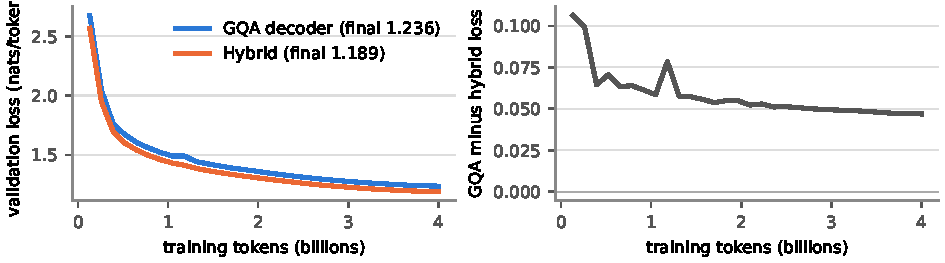
\includegraphics[width=\textwidth]{pretrain_val.pdf}
\caption{Phase 1 validation loss for the GQA decoder and the hybrid on the same data order (left), and the gap between them (right). The hybrid needed about 20\% fewer tokens to reach GQA's loss at step 1,250, and finished 0.047 lower.}
\label{fig:pretrain}
\end{figure}

For \textbf{Phase 1}, the hybrid's validation loss stayed lower than GQA's at every check (Figure~\ref{fig:pretrain}), where the gap peaked at 0.106 and narrowed to 0.047 at 4.0B tokens, and when I tested the new GQA model offline on 60 official prompts with our own ROUGE, greedy decoding looped in 86\% of outputs and blocking repeated 3-grams took ROUGE-L from 0.216 to 0.226 ahead of nucleus sampling (0.213) and a repetition penalty (0.203), though as that only barely beat copying the prompt's last 128 words (0.198) we never submitted those continuations; across \textbf{Phases 2--6}, ensembling in Phase 2 added only 0.006 over GQA alone and in Phase 3 context mattered most as the sentence window added about 10 points of test macro-F1, in Phase 4 the ensemble fixed before test (0.5992) beat the pair picked on dev (0.5912), in Phase 5 the gain came from scaled-up pretraining and the TF-IDF blend, not the architecture, and in Phase 6 shorter summaries scored better (ratio 0.18 beat 0.22), beam search added 0.0053 on test with six beams no better than four, and our final context split got the highest BERTScore even as test ROUGE-1 dropped from 0.484 to 0.459, so the two metrics disagree.

In \textbf{Phase 7}, our top submission got 0.4938 Micro-F1@7 (precision 0.5039, recall 0.4841), where only the learned ranker gave a clearly significant jump (+0.0245 dev, interval [0.0095, 0.0410]) and the citing-sentence features added +0.0100 ([$-0.0010$, 0.0214]) alongside +0.0044 ([0.0010, 0.0094]) from the rerankers, worth about eight test hits with the blend weight picked from about 15 dev trials; as for \textbf{what won and why}, in the classification tasks what worked best was feeding the right part of the case into a well-trained backbone and combining it with a lexical baseline, as the 214M checkpoints helped because they saw 30 times more legal material whereas the hybrid's lower pretraining loss did not turn into a downstream edge, and for retrieval exact word overlap did the heavy lifting because citing judgments quote the cases they cite, which word 4-gram overlap picks up directly whereas a 1,024-token neural excerpt only partly retains it.
% ============================================================
\section{Error Analysis and Discussion}\label{sec:errors}
% ============================================================
\subsection{Phase-wise failure modes}
For \textbf{Phase 2}, the ensemble gain over GQA alone was small (0.5443 against 0.5388), running GQA from 6 to 15 epochs added only 0.003, and LoRMA got 0.0155 (far below every other run, pointing to a broken export rather than a weak model, though we did not resubmit it); two things in the data also cap strict F1, namely 26 surface strings taking different labels in different cases (``Union of India'' as appellant, respondent or authority) which only document context resolves and 137 entity pairs touching with only whitespace between them where one boundary slip ruins two spans, with counsel, judge and witness each under 3\% of entities yet weighing one twelfth of macro-F1. On \textbf{Phase 3}, copying the previous gold label gets 0.749 so roles are sequential, yet sequence models on cheap features did not help as Viterbi decoding with transition counts pulled TF-IDF down from 0.396 to 0.31--0.35 and a document-level BiLSTM-CRF got 0.347; capping sentences at 63 tokens cut 18--22\% of them, runs overfitted fast (one distillation run hit 0.99 train F1 as dev loss doubled), and three later runs got 0.4294--0.4386 on test despite reaching 0.4942 on dev because 10 dev docs are too few. During \textbf{Phase 4}, dev-tuned thresholds did not transfer (overstating run 1 by 4.7 points), run 9 had the highest dev F1 among controls (0.6122) yet the lowest test F1 (0.5648), and every neural run stayed at or below TF-IDF on dev, whereas rare statutes are the weak spot in \textbf{Phase 5} with mean F1 by training-frequency quartile rising from 0.23 and 0.33 to 0.36 and 0.50. Because \textbf{Phase 6} BERTScore truncates both texts at 512 RoBERTa tokens, only about the first 400 words count even though test references average 932 words, so text past that cutoff is not scored (which is why shorter outputs and more summary context helped) and a no-repeat size of 6 let the decoder loop via paraphrase (13\% repeated word 4-grams). Finally, in \textbf{Phase 7}, 449 of 973 dev gold cases were retrieved and 417 cannot be as their queries cite more than seven; recall drops from 0.68 to 0.23 on longer queries, but hits over available slots rise from 0.65 to 0.90 so long queries are not harder, leaving citation without shared text as the main error (missed gold cases average an overlap z-score of 0.56 against 3.37 for hits, and the neural term swapped only 58 of 826 top-7 entries, 21 gold gained and 17 lost, as its excerpts come from the same n-gram overlap, which may limit it to evidence the lexical stage already has).

\subsection{What the metrics do not measure}
In practice I found that ROUGE and BERTScore reward overlap with one reference, not legal accuracy, meaning a summary can score high after dropping the holding and BERTScore ignores text past about 400 words, just as strict span F1 gives no credit if a right entity is off by one character, statute macro-F1 weights rare and common statutes equally (noisy on sparse test statutes), and Phase 7 gold labels track citation, not relevance, counting uncited relevant cases as errors.

\subsection{Limitations and what you would do next}
As most comparisons use one seed and test splits are small (one Phase 7 hit shifts test F1 by about 0.0006), small gaps are not resolvable, and our models read at most 2,048 tokens of judgments that often exceed 10,000, our leakage check never covered Phases 2 and 3, and no lawyer checked the outputs; next, we would score several chunks per Phase 7 candidate so the reranker sees text the lexical stage did not pick up, weight the Phase 6 loss towards the window BERTScore scores, and use the hybrid's recurrent state to read full judgments in Phases 4 and 5.

\subsection{Surprising findings}
Looking back, three findings went against expectations, as the hybrid's lower pretraining loss never turned into a measurable downstream edge, our strongest standalone reranker in Phase 7 was the worst model in the blend even as a frozen backbone blended as well as a fine-tuned one, and a position-only cue (where citations sit in the query) gave more test hits than any neural model (about 17 against 8).
% ============================================================
\section{Conclusion}
% ============================================================
Two choices actually moved our scores, namely retraining the base model on 30 times more legal material and pairing our neural models with lexical baselines (TF-IDF in Phase 5, plus n-gram overlap and a learned ranker in Phase 7), and in Phase 6 tuning decoding for the window the metric scores also helped. As the choice of backbone and tuning method did not measurably matter, parameter-efficient adapters that cut memory in half are our default, and the takeaway for a compact legal model under a parameter and data cap is that token budget and honest evaluation matter more than architecture whereas exact word overlap remains the strongest signal on long judgments.

\newpage
% ============================================================
\section*{LLM Usage Declaration}
% ============================================================
\noindent
\textbf{Q1.} Which Large Language Model(s), if any, did you use while completing the competition or writing this report? \\[0.4em]
Answer: Claude (Anthropic), from Phase 3 onwards and for this report; ChatGPT (OpenAI) in the earlier phases.
\medskip

\noindent
\textbf{Q2.} For each row, mark Yes or No and state the purpose in one short phrase.
\begin{table}[H]
\centering\small
\begin{tabular}{>{\raggedright\arraybackslash}p{4.6cm}|c|>{\raggedright\arraybackslash}p{7.2cm}}
\toprule
Part & Used LLM? & Purpose of using the LLM \\
\midrule
Understanding concepts / papers & Yes & Explaining LoRMA, Mamba-2, BERTScore and bootstrap tests \\
Ideation / brainstorming at a high level & Yes & Proposing experiments and controls \\
Debugging small ancillary snippets & Yes & Fixing notebook and evaluation bugs \\
Plotting / visualization code & Yes & Figure scripts \\
Grammar / writing style of the report & Yes & Editing prose \\
Report structure / section wording & Yes & Drafting sections from our results \\
Designing the model architecture & Yes & Implementing the Hymba-style hybrid and encoder \\
Hyperparameter search / tuning & Yes & Generating sweep configs and logging scripts \\
Analysis of results / conclusions & Yes & Formatting result tables and statistical test scripts \\
Writing the core training / inference code & Yes & Generating boilerplate training and inference script stubs \\
Other (specify) & Yes & Packaging submission archives and checking file formats \\
\bottomrule
\end{tabular}
\end{table}
\medskip

\noindent
\textbf{Q3.} Did you refer to sources other than lecture slides and an LLM? \\[0.4em]
Answer: Yes: the papers in the bibliography, the course scaffold code and starter notebooks, the official evaluation scripts, and the documentation of PyTorch, scikit-learn and the \texttt{bert-score} package.
\medskip

\noindent
\textbf{Q4.} Apart from any permitted LLM use, what was \emph{your} contribution? \\[0.4em]
I drove the experimental design, architecture choices, debugging decisions and evaluation protocol across all seven phases, using the LLMs to generate code stubs, sweep configurations and draft text that I verified and ran across our Colab sessions. Specifically, after running the Phase 4 frozen-feature probe and seeing that our initial 63--67M models (0.562 dev macro-F1) barely beat random weights (0.514) and trailed TF-IDF (0.612), I diagnosed the issue as severe token under-training from equal-source sampling and initiated the 27 October restart, scaling to three matched 214M-parameter architectures trained on 4.0B tokens in natural corpus proportions. I also benchmarked throughput on Colab and dropped the 56k tokens/s latent-attention decoder in favour of the 130k tokens/s GQA backbone, designed the three-stage Phase 7 retrieval pipeline (hashed word 4-gram overlap, a 27-feature LightGBM ranker with citing-context features, and three neural rerankers) that reached 0.4938 Micro-F1@7 (Rank 8 of 121), and ran the two-fold cross-fit threshold shrinkage ($m=30$) in Phase 5 and paired query bootstrap tests in Phase 7. I enforced strict evaluation hygiene throughout: when we discovered that residual citation traces survived the organizers' \texttt{<CITATION>} masking in Phase 7 and raised dev F1 from 0.4603 to 0.4747, I refused to submit that run because it exploited a masking leak rather than improving the model. Managing the Colab runs, checkpoint restarts and all 87 Codabench submissions myself also surfaced two key experimental lessons: in Phase 4, dev-tuned thresholds overstated test by 2.5 points due to overfitting on a small split, and in Phase 7 the reranker trained with random negatives scored best standalone (0.3391) yet worst in the blend because its predictions correlated 0.555 with the lexical ranker.

\vspace{1em}
\bibliographystyle{ieeetr}
\bibliography{references}
\end{document}
